\documentclass[12pt]{report}
\usepackage{amsmath,amssymb,amsfonts}
\usepackage{courier}
\usepackage{graphicx}
\usepackage{hyperref}
\usepackage{listings}
\usepackage{color}
\usepackage{tikz}
\usepackage{circuitikz}
\usetikzlibrary{shapes,arrows}
\usepackage[margin=2cm]{geometry}

\title{ECSE 426 - Microprocessor Systems\\Lab Report 1: Analog Data Acquisition, Filtering, and
Digital I/O}
\author{Harley Wiltzer (260690006)\\Matthew Lesko (260692352)}
\date{February 19, 2018}

\definecolor{dblue}{rgb}{0.4,0.4,0.8}

\hypersetup {
	colorlinks=true,
	linkcolor=dblue
}

\tikzstyle{decision} = [diamond, draw, fill=blue!20, text badly centered, text width=2cm, node
distance=3cm]
\tikzstyle{block} = [rectangle, draw, fill=blue!20, text centered, rounded corners, minimum
height=4em, text width=3cm, node distance=5cm]
\tikzstyle{goal} = [rectangle, draw, fill=yellow!20, text centered, rounded corners, minimum
height=4em, text width=3cm, node distance=5cm]
\tikzstyle{line} = [draw, -latex']
\tikzstyle{cloud} = [draw, ellipse, fill=red!20, node distance=7cm, text centered, text width=2cm]
\tikzstyle{label} = [draw, rectangle, text centered, text width = 3cm]

\renewcommand*\thesection{\arabic{section}}

\begin{document}
\maketitle
\pagenumbering{roman}
\tableofcontents
%\let\clearpage\relax
\listoffigures
\let\clearpage\relax
\listoftables
\newpage
\pagenumbering{arabic}
\section{Abstract}
The purpose of the experiment is for the programmers to get exposure to analog data acquisition and
data conditioning on the STM32F4 board. The programmers will get familiar with the STM32CubeMX application, the HAL
software libraries in embedded C, specifically for analog to digital signal conversion on the
STM32F4 Discovery board and the I/O interface for buttons, LEDs and a 7-segment display on the
board. Ultimately, with these tools, the programmers will demonstrate the design and construction of
a voltmeter. This report will explain how the programmers configured their project and implemented the
task mentioned below, as well as explain the challenges faced, the data
encountered while testing and debugging, and the conclusions made. By the end of the report, the reader will have understood how the data acquisition and conversion tools available on the STM32F4 board could be used to create an effective voltemeter.
\section{Problem Statement}
The problem of the experiment is for the programmers to implement a solution for converting an analog signal to digital, filtering samples of the signal at a certain sampling frequency, calculating RMS, max, and min values, and finally displaying the calculated values on a 7-segment display with the help of a button for switching values. With the final product being a working and effective voltemeter.
As mentioned in the experiment 2 handout [1], solving the problem involves the following steps:
\begin{enumerate}
  \item Setting up the blue button;
  \item Setting up a DAC;
  \item Setting up an ADC;
  \item Setting up the sampling frequency;
  \item Signal filtering;
  \item Making sense of data;
  \item Configuring the voltage display;
\end{enumerate}
For any specific details about the required steps, please refer to the experiment 2 handout [1].\\
The task had multiple challenges that the developers had to solve.
Firstly, the programmers faced challenges with properly configuring the project with the STM32CubeMX
application. One had to understand and correctly use the HAL libraries, specifically for its ADC and
DAC functions. There were problems with configuring the SysTick properly, such as choosing the
correct frequency. Furthermore, the developers had to implement a solution for the blue button to
act as an interrupt as opposed to continuously reading values when it was held down as well as
having had to map appropriate GPIO and ADC pins on the board to the code written in the Keil IDE. As
for calculating the RMS, max, and min values, there had to a solution for calculating these values
without storing 10 second records which provided increased difficulty. Finally, designing a circuit
for the 7-segment display on the bread board without damaging the display or the microcontroller
proved to be a challenge to the programmers.
\section{Theory and Hypothesis}
\subsection{System Clock}
As mentioned in the second tutorial handout, the micro-controller has two sources of clock, an internal one and an external one which could be more accurate with the use of a crystal working at 8 MHz [2]. This clock determines the frequency of each other clock configured within the system. For this experiment, the RCC's High Speed Clock pin is mapped to the external crystal.
\subsection{ADC Clock}
Microcontrollers can detect binary signals, but real-world signals are not as simple, programmers must deal with voltages such as 2.72V, 3.33V, etc. as opposed to just a binary decision of 0 or 1V. The STM32F4 Discover board has an ADC feature, governed by a clock, that allows one to convert analog signals to digital. To understand the ADC feature, one must first comprehend its sampling frequency.
By having the programmers determine the system's clock (SYSCLK), the ADC's clock is determined by the following procedure [3]:\\
\[ AHBCLK = SYSCLK * AHBPRESC (/1, 2, ..., 512)\\ \]
\[ APB2CLK = AHBCLK * APB2PRESC (/1, 2, 4, 8, 16)\\ \]
\[ ADCCLK = APB2CLK * ADCPRESC (/2, 4, 6, 8)\\ \]
The prescalers are parameters that configure the system's multiple clocks, it is up to the designer to select the parameters. While there are multiple clocks, the important one to notice is the ADCCLK. The ADC's clock determines the ADC's sampling frequency.\\
The total conversion time of the ADC is determined by solving the following equation [3]:\\
\[ Total Conversion Time = T_{Sampling} + T_{Conversion} \]\\
One can find the conversion time (\(T_{Conversion}\)) by cross referencing the resolution to its respective amount of cycles within the time conversion table[3].\\
\begin{table}[h]\label{adcres}
	\caption{Resolution Time Conversion Table}
	\begin{center}
		\begin{tabular}{|c|c|}
		\hline
		Resolution (bits) & Conversion Time (cycles)\\\hline
		12 & 12 \\\hline
		10  & 10 \\\hline
		8  & 8 \\\hline
		6  & 6 \\\hline
	\end{tabular}
	\end{center}
\end{table}
The sampling time (\(T_{Sampling}\)) is determined by the channel chosen for the ADC's clock. Possible sample times are 3, 15, 28, 58, 84, 112, 144, and 480 cycles [3].\\
Finally, one can derive the sampling frequency using the following equation:
\[ Sampling Frequency (sps) = (1/ADCCLK * (Total Conversion time))^{-1} \]
By knowing the sampling frequency, a designer can determine the number of samples obtained within a certain period and base their calculations for measurements from that.\\
\subsection{ADC Component}
There are many ways of implementing the ADC, but this report will go into detail about the theory
for the ADC used in this experiment [4]. The voltages used across the ADC include the following:\\
\begin{itemize}
	\item \(V_{IN}\): The voltage of the analog input;
	\item \(V_{REF}\): Reference voltage fed to the ADC; 
\end{itemize}
The N-Bit register is first configured midscale, in which the MSB is 1, and all other bits are zeros. The length of the bit string stored in the N-Bit register is the number of bits chosen for the ADC's resolution.\\
\begin{figure}\label{adc}
	\begin{center}
		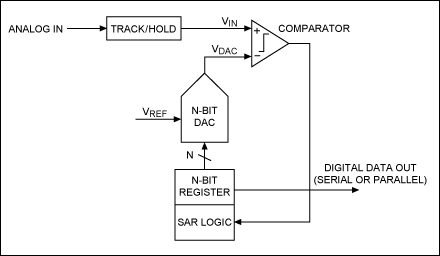
\includegraphics{adc.png}
		\caption{SAR ADC Architecture [4]}
	\end{center}
\end{figure}

The comparator component outputs a logic high (1) if $V_{IN}$ is greater than $V_{DAC}$ or a logic low (0)
otherwise. If the comparator's output is high, then the SAR (Successive-Approximation-Register) does
not change the current bit in the N-bit register, which is by default a 1. The SAR then moves down
the bit string, changes the current bit to a 1, and allows for another comparison. If the
comparator's output is low, the SAR forces the current bit in the N-bit register to a 0 and moves
down to the next bit, changes the current bit to a 1, then allows for another comparison. This
process is done until the N-bit digital word is available in the register. By the end, the ADC has
successfully converted an analog input to a digital word. In the case of this experiment, since the
resolution is of 8 bits, the ADC would create 8-bit digital words.
\subsection{Push-Pull and Open-Drain Output Stages}
The open-drain output pin is driven by a single transistor as opposed to two in the push-pull output stage. There are two states for the open-drain output pin. When the output device is off, the pin has a floating voltage and when it is on, the transistor pulls the input signal to ground [5].
A push-pull output stage has two transistors. One transistor dissipates the current from the load to ground or a negative supply, and the other supplying current to the load from a power supply [6]. The outputs of open-drain and push-pull accept all ranges of voltages within 0 to 3.3V [2]. 
\subsection{Signal Filtering}
The filter used for this experiment is identical to the one from experiment \#1. The implementation of the filter is simple. The filter holds five single-precision floating-point numbers and uses a technique called Moving Average to compute the average of the coefficients. The technique stores the last five inputs which are used again when a new input is passed to the filter.
\subsection{Hypothesis}
The programmers should be able to implement a solution for the problem at hand, since the majority of the experiment requires understanding and proper utilization of the STM32F4 discover board configurations and components which is doable within the given time frame of two weeks. The hardest challenge would be debugging problems with the ADC and the circuitry for the 7-segment display. Having done previous laboratories with electric circuit components, the programmers should be able to design a circuit for the 7-segment display.

\section{Implementation}
The design of the voltmeter was fairly complex and was composed of several modules.
These modules included the \hyperref[userinput]{user input module} for processing user input via the
push button, the \hyperref[dataaq]{data
acquisition module} for digitizing analog data on the board, the \hyperref[dataproc]{data processing
module} for filtering
the data and associating meaning to its digital values, and the \hyperref[output]{output module} for
displaying the
data to the user. This section will be divided into several subsections, each corresponding to a
module, in order to organize the design decisions that were made.\\\\
Since all of these modules needed to work together, they had to be synchronized
appropriately, and this was achieved with the \texttt{SysTick} timer. The \texttt{SysTick} timer
invokes interrupts at a chosen frequency, and the interrupt handler was used to coordinate all of
the modules. Since the configuration parameters of the \texttt{SysTick} timer were heavily
influenced by the modules described above, they will be explained independently in the sections
following where the design decisions were made. Specific details concerning the configuration
parameters of the \hyperref[appendixgpio]{GPIO pins}, the \hyperref[appendixadc]{ADC}, and the
\hyperref[appendixdac]{DAC} may be perused in the appendices. Furthermore,
\hyperref[mammoth]{Appendix E} contains all GPIO configuration code generated by the HAL Cube MX
software for this project.
\subsection{High Level System Architecture}
The figure below shows how the major components of the system were organized.\\\\
\begin{figure}\label{systemarc}[h]
	\begin{center}
		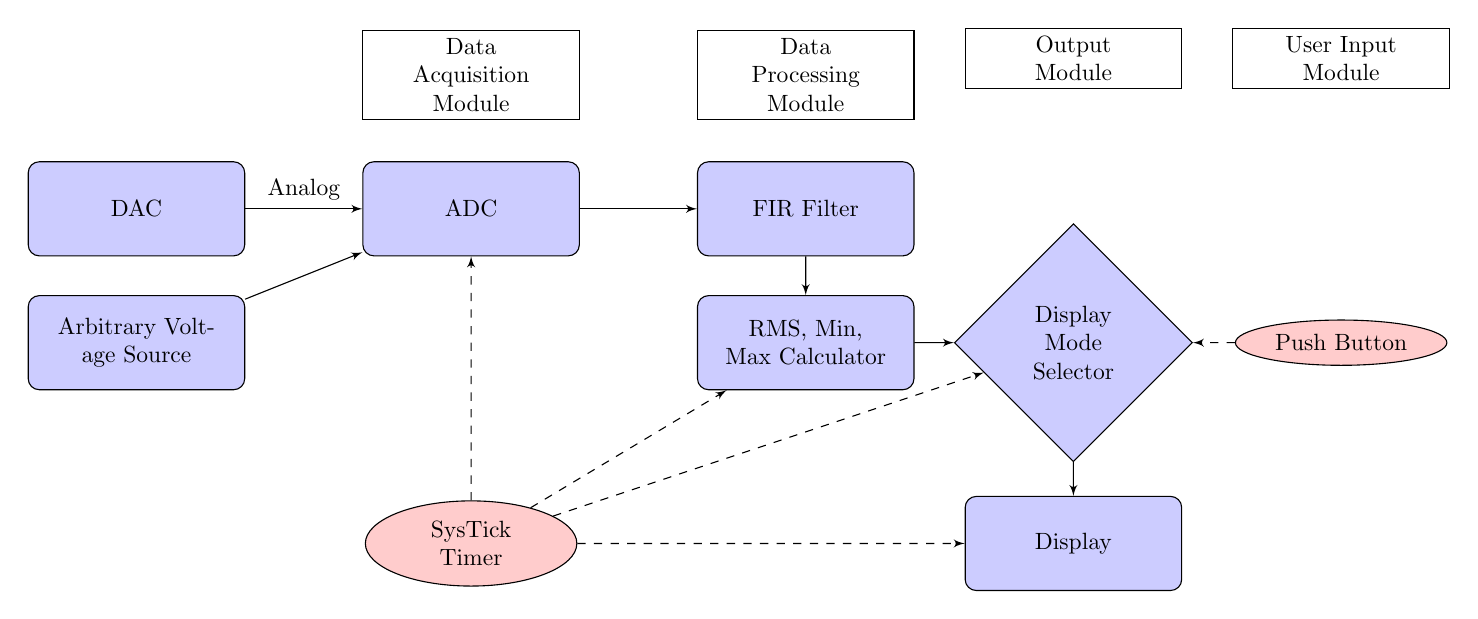
\begin{tikzpicture}[node distance = 2cm, auto, scale=0.85, transform shape]
			\node [block] (dac) {DAC};
			\node [block, below of=dac, node distance=2cm] (volts) {Arbitrary Voltage Source};
			\node [block, right of=dac] (adc) {ADC};
			\node [cloud, below of=adc, node distance=5cm] (systick) {SysTick Timer};
			\node [block, right of=adc] (filter) {FIR Filter};
			\node [block, below of=filter, node distance=2cm] (process) {RMS, Min, Max Calculator};
			\node [decision, right of=process, node distance=4cm] (select) {Display Mode Selector};
			\node [cloud, right of=select, node distance=4cm] (button) {Push Button};
			\node [block, below of=select, node distance=3cm] (display) {Display};
			\node [label, above of=adc] (adclabel) {Data\\Acquisition\\Module};
			\node [label, above of=filter] (filterlabel) {Data\\Processing\\Module};
			\node [label, above of=select, node distance=4.25cm] (displaylabel) {Output\\Module};
			\node [label, above of=button, node distance=4.25cm] (buttonlabel) {User Input\\Module};
			\path [line] (dac) -- node {Analog} (adc);
			\path [line] (volts) -- (adc);
			\path [line, dashed] (systick) -- (adc);
			\path [line] (adc) -- (filter);
			\path [line] (filter) -- (process);
			\path [line] (process) -- (select);
			\path [line] (select) -- (display);
			\path [line,dashed] (button) -- (select);
			\path [line,dashed] (systick) -- (select);
			\path [line,dashed] (systick) -- (display);
			\path [line,dashed] (systick) -- (process);
		\end{tikzpicture}
		\caption{System Architecture}
	\end{center}
\end{figure}
Figure 2 shows the overall architecture of the voltmeter system, organized in columns by the modules
that each component belong to. The remainder of this section will discuss in more detail how each of
these modules were designed.
\subsection{The User Input Module}\label{userinput}
One of the requirements of the voltmeter was to provide three display modes to the user: a display
of the RMS voltage, and a display for each of minimum and maximum voltage updated within the past
ten seconds. As such, there was a need for user input to switch between these display modes. This
was achieved with the user button on the STM32F407 board, which allowed the user to cycle through
each of the display modes by pressing the button.\\\\
The first challenge dealt with how to process the button presses. There were two main options:
polling for button presses and handling interrupts. Since polling the button at every iteration in a
loop seemed inefficient, the interrupt method was chosen. Therefore, an NVIC interrupt was
configured at priority 0 for \texttt{EXTI0}. However, even with the interrupts set up, there was
still a major challenge to correctly process the button presses, as one button press often caused
several interrupts. This could have been do to button bouncing, or possibly the fact that a what
seems like a short \textit{click} to a human actually goes over several clock cycles of the
processor. To prevent this from occuring, it was decided to enforce a time delay between consecutive
button press handling routines, and this was achieved using the \texttt{SysTick} timer. The process
is shown in \hyperref[buttonflow]{Figure 3}.\\\\
\begin{figure}\label{buttonflow}
	\begin{center}
		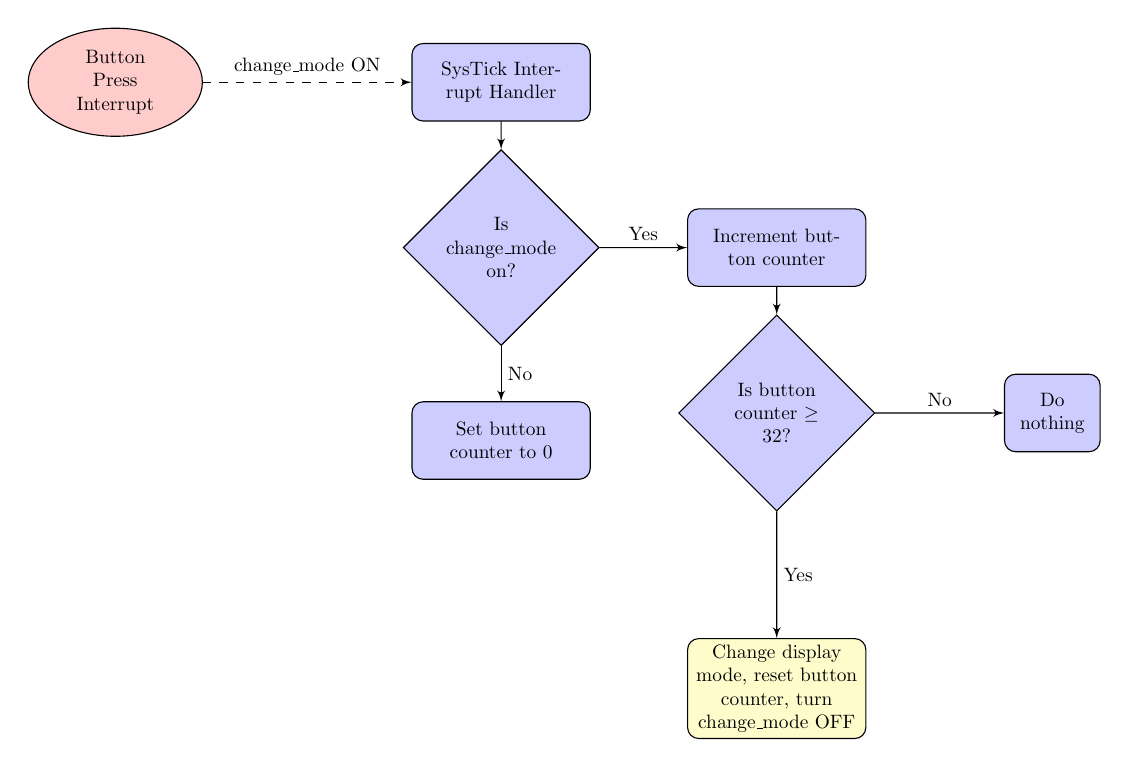
\begin{tikzpicture}[node distance = 2cm, auto, scale=0.7, transform shape]
			\node [block] (tick) {SysTick Interrupt Handler};
			\node [cloud,left of=tick] (exti0) {Button Press Interrupt};
			\node [decision, below of=tick] (ifchange) {Is change\_mode on?};
			\node [block, below of=ifchange, node distance=3.5cm] (zerobc) {Set button counter to 0};
			\node [block, right of=ifchange, node distance=5cm] (incbc) {Increment button counter};
			\node [decision, below of=incbc] (ifcount) {Is button counter $\geq$ 32?};
			\node [block, right of=ifcount, text width=1.5cm] (wait) {Do nothing};
			\node [goal, below of=ifcount] (button) {Change display mode, reset button counter, turn
			change\_mode OFF};
			\path [line, dashed] (exti0) -- node {change\_mode ON} (tick);
			\path [line] (tick) -- (ifchange);
			\path [line] (ifchange) -- node {No} (zerobc);
			\path [line] (ifchange) -- node {Yes} (incbc);
			\path [line] (incbc) -- (ifcount);
			\path [line] (ifcount) -- node {No} (wait);
			\path [line] (ifcount) -- node {Yes} (button);
		\end{tikzpicture}
		\caption{Debouncing button presses}
	\end{center}
\end{figure}
\textit{In brevarium}, the \texttt{EXTI0\_IRQHandler()} function (invoked by the button press
interrupt) asserts a \texttt{change\_mode} signal, and when the \texttt{SysTick\_Handler()} function
(invoked by \texttt{SysTick} interrupt) sees that, it waits for 32 consecutive \texttt{SysTick}
interrupts before taking action. The number 32 was achieved via trial and error, as it was unknown
exactly how long an average human button press lasts. That being said, this number was chosen at a
\texttt{SysTick} frequency of 200Hz, so a delay of 160ms was imposed.

\subsection{The Data Acquisition Module}\label{dataaq}
The data acquisition module was responsible for gathering analog data and digitizing it so it could
be processed. Firstly, however, it was helpful to set up a digital to analog converter (DAC) in
order to test the performance of the analog to digital converter (ADC). Setting up the DAC was
fairly straightforward, and most of the work was carried out by the HAL Cube software. The DAC was
configured on channel 1, and it wrote to pin PA4 on the board. Furthermore, its resolution had to be
chosen. Since the performance of the voltmeter ultimately depended on the resolution of the ADC, the
resolution of the DAC was chosen to be the same as that of the ADC, which was 8 bits, right aligned.
This decision will be explained when discussing the ADC parameters below. Finally, the DAC needed to
output some analog voltage. A value was chosen arbitrarily and passed to the DAC via the
\texttt{HAL\_DAC\_SetValue()} driver function, and the conversion was instantiated via
\texttt{HAL\_DAC\_Start()}. This starts a conversion in polling mode, which was deemed appropriate
for the purposes of this experiment as the conversion would only occur once.\\\\
Setting up the ADC was considerably more complicated. Again, the basic initialization was done by
the HAL Cube software, and the ADC1 unit was set up on channel 1. Single conversion mode was chosen,
as it was required for one conversion to occur at a given frequency. Once again, the resolution had
to be determined. Since it was known that the displayed voltages would be shown with two decimal
places of precision, the user could only see voltages in increments of $0.01$V. 
\begin{table}[h]\label{adcres}
	\caption{Accuracy of ADC by resolution}
	\begin{center}
		\begin{tabular}{|c|c|}
			\hline
			Resolution (bits) & Voltage difference between consecutive digital values (V)\\\hline
			6 & 0.047\\\hline
			8 & 0.012\\\hline
			10 & 0.003\\\hline
			12 & 4.89e-4\\\hline
		\end{tabular}
	\end{center}
\end{table}
The accuracy of the ADC by its resolution is shown in \hyperref[adcres]{Table 1}. The accuracy is
defined here as the change in voltage when increasing the digital reading by 1. Since the voltage
range of the ADC is 3V, the accuracies were calculated according to
\begin{equation}
	A = \frac{3}{2^{R}}
\end{equation}
were $A$ is the accuracy (rightmost column) and $R$ is the resolution (leftmost column). Clearly, a
resolution of 6 bits is not a great choice, as it cannot resolve voltages within 0.047V from each
other. Since the display of the voltmeter allowed two decimal places, this accuracy is insufficient.
With a resolution of 10 bits, however, the accuracy is relatively high. At an accuracy of 0.003V,
the display would only change after a change of 4 in the digital reading of the ADC. The 8 bit
resolution could resolve voltages that are 0.012V apart which is very close to the accuracy on the
display. Ultimately, the 8 bit and 10 bit resolutions were the main contenders, because the 8 bit
resolution is slightly worse than that of the display, and the 10 bit resolution is much stronger
than that of the display. In the end, the 8 bit resolution was chosen as it was deemed strong enough
for the purposes of this experiment, it would cause lower power consumption, and it matched one of
the possible resolutions of the DAC which made the code simpler.\\\\
Next, the conversion mode of the ADC had to be chosen. Polling mode was not considered a viable
option, since ADC conversions would happen frequently and thus polling would waste a considerable
portion of the CPU's cycles. Although DMA was a very good alternative, the developers did not have
time to do the requisite research. Therefore, interrupt mode was selected. Despite the conversion
mode, however, the frequency of ADC conversions remained to be implemented. A sample rate of 50Hz
was required, so the \texttt{SysTick} interrupts were used to time the ADC conversions. Since the
\texttt{SysTick} interrupts were occuring at 200Hz (see the \hyperref[output]{Output subsection} below), it was
required to implement a prescaler in the \texttt{SysTick\_Handler()} function in order to sample at
50Hz.
\begin{figure}[h]\label{adcflow}
	\begin{center}
		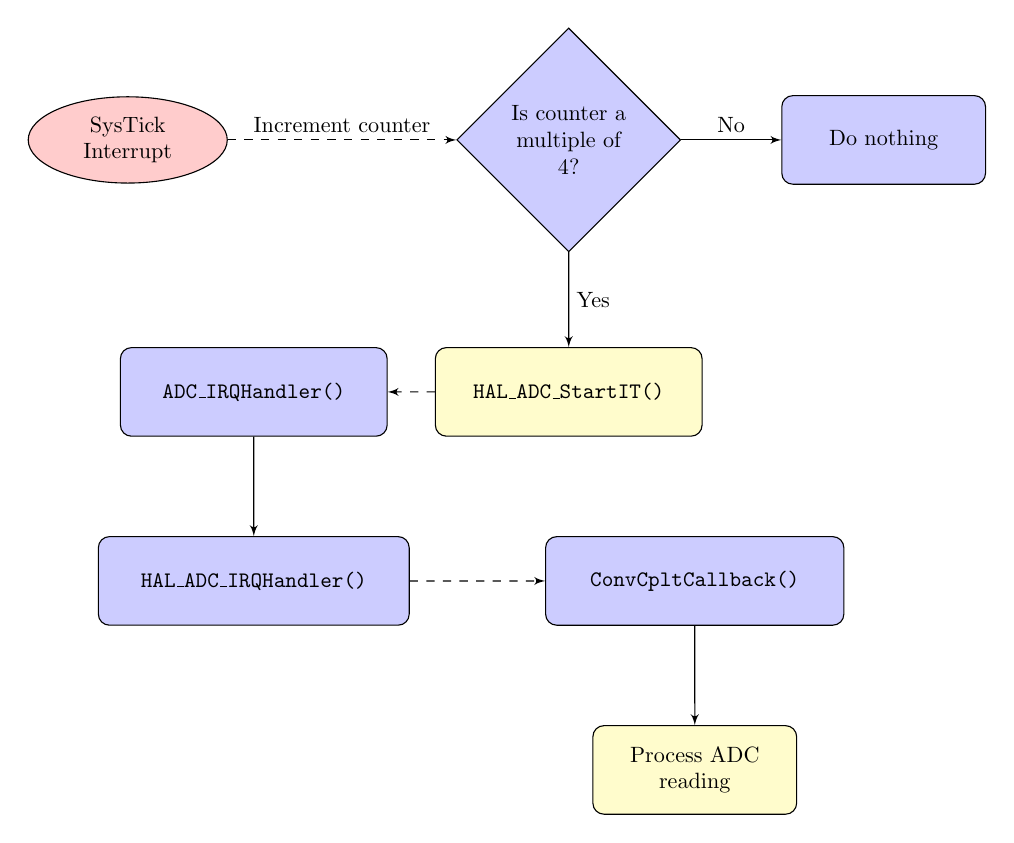
\begin{tikzpicture}[node distance=2cm, auto, scale=0.8, transform shape]
			\node [cloud, node distance=7cm] (systick) {SysTick Interrupt};
			\node [decision, right of=systick,node distance=7cm] (ifcount) {Is counter a multiple of 4?};
			\node [block, right of=ifcount] (nothing) {Do nothing};
			\node [goal, below of=ifcount, text width=4cm, node distance=4cm] (startadc) {\texttt{HAL\_ADC\_StartIT()}};
			\node [block, left of=startadc, text width=4cm] (irqhandler) {\texttt{ADC\_IRQHandler()}};
			\node [block, below of=irqhandler, text width=4.7cm, node distance=3cm] (haladc)
			{\texttt{HAL\_ADC\_IRQHandler()}};
			\node [block, right of=haladc, text width=4.5cm, node distance=7cm] (conv) {\texttt{ConvCpltCallback()}};
			\node [goal, below of=conv, node distance=3cm] (processadc) {Process ADC reading};
			\path [line, dashed] (systick) -- node {Increment counter} (ifcount);
			\path [line] (ifcount) -- node {No} (nothing);
			\path [line] (ifcount) -- node {Yes} (startadc);
			\path [line, dashed] (startadc) -- (irqhandler);
			\path [line] (irqhandler) -- (haladc);
			\path [line, dashed] (haladc) -- (conv);
			\path [line] (conv) -- (processadc);
		\end{tikzpicture}
		\caption{Flow of ADC processing}
	\end{center}
\end{figure}
The process of handling ADC conversions is shown in \hyperref[adcflow]{Figure 4}. The
\texttt{SysTick\_Handler()} maintains a \texttt{counter} and increments it at every \texttt{SysTick}
interrupt, that is to say, at 200Hz. Since ADC conversions were to be taken at 50Hz, they had to be
triggered at a rate four times less frequent than \texttt{SysTick}. Thus, the
\texttt{HAL\_ADC\_StartIT()} function was called on every fourth \texttt{SysTick} interrupt to start
ADC conversions at 50Hz. This was accomplished by starting the ADC conversion when the
\texttt{counter} variable was a multiple of 4.

\subsection{The Data Processing Module}\label{dataproc}
Given the digital readings from the ADC, the next step was to filter them to reduce noise and to
then translate the readings into meaningful values. These steps were carried out in the
\texttt{ConvCpltCallback()} function (see \hyperref[adcflow]{Figure 4}). In order to reduce noise,
the digital readings
were passed through a $4^{th}$ order FIR filter, which effectively output the average over the past
5 inputs. A $9^{th}$ order filter was experimented (which effetively output the average over the
past 10 inputs), but it had a negligible effect on the performance of the voltmeter. Since the
$9^{th}$ order filter required considerably more memory, the $4^{th}$ order filter was chosen. By
passing each new ADC reading through the filter, potential noise will be ``smoothed out", as it will
be converted into the average of that reading and the previous 4.\\\\
Upon filtering the ADC readings, the filtered output was then translated into its analog
representation according to
\begin{equation}
	x_a = V_{DD}\left (\frac{\mathcal{F}(x_d)}{2^{R} -1}\right)
\end{equation}
where $x_a$ is the analog representation of the new ADC reading, $\mathcal{F}(x_d)$ is the filtered
digital ADC reading, $R$ is the resolution (in bits) of the ADC, and $V_{DD}$ is the highest voltage
that the ADC is rated for. Finally, the analog value is passed to the \texttt{plot\_point()}
function, which is responsible for curating the inputs into the form in which they should be
displayed.\\\\
The goal of the \texttt{plot\_point()} function is to maintain the values of the RMS voltage over
the past 10 seconds, as well as the minimum and maximum voltages over the past 10 seconds, while
making efficient use of memory. It was decided to design this in a ``moving window" fashion, meaning
the values to be displayed will always taken into account data from within the past 10 seconds, and
not in discrete 10 second blocks. With the requirement of keeping memory usage down to at most 20
samples, this was a difficult task. Firstly, it was decided that the minimum and maximum voltage do
not need to be updated very frequently. Of the 20 samples, 5 samples were allocated to each of
minimum and maximum voltages, and the remaining 10 samples were reserved for RMS voltage. With only
5 samples for each of minimum and maximum voltages, each sample would have to represent the minimum
or maximum sample in a 2 second interval. Likewise, for RMS, each stored sample represents the
running RMS over a 1 second interval. The minimum samples, maximum samples, and RMS samples were
each stored in their own circular list (see \hyperref[circularlists]{Appendix A}) for efficient
insertion and removal. For each 100 samples (2
seconds) passed to \texttt{plot\_point()}, the minimum and maximum were calculated and added to their
respective circular lists. For the RMS calculations, a new value was added to the RMS circular list
for every 50 samples (1 second), however the value to be added could not be the RMS exactly. RMS is
calculated as follows
\begin{equation}
	\mathsf{RMS} = \sqrt{\frac{1}{|N|}\sum_{n\in N}n^2}
\end{equation}
where $N$ is the set of samples to calculate the RMS over. Since the square root operation is
nonlinear, the RMS itself cannot be passed to the RMS circular list every second. Rather, the
\textit{sum of squares} $\sum_{n\in N'}n^2$ is passed, and the RMS is calculated over the past 10
sum of squares values.\\\\
With the circular lists mentioned above, the \texttt{plot\_point()} function was able to return the
RMS, minimum, and maximum voltages over the past 10 seconds fairly easily. For the minimum and
maximum voltages, this consisted of simply finding the minimum value in the minimum voltages circular
list and the maximum value in the maximum values circular list. The RMS over the past 10 seconds was
computed as follows:
\begin{equation}
	\mathsf{RMS}_{10} = \sqrt{\frac{1}{50|S|}\sum_{s\in S}s}
\end{equation}
where $S$ is the set of the 10 most recent second-long sum of squares calculations described above.
Since each second consists of 50 readings, the sum of sums of squares had to be divided by $50|S|$,
because it summed over 50 points for each $s\in S$.\\\\
Note that although the RMS is only being updated once per second and the minumum and maximum are
only being updated once every 2 seconds, the circular lists still store enough data to report the
exact RMS, minimum, and maximum over a moving 10 second window. Due to the constraint on memory
usage, the update frequency of the RMS, minimum, and maximum could not be improved with a moving
window design.

\section{The Output Module}\label{output}
The output module was responsible for displaying the data that the \hyperref[dataproc]{data
processing module} computed using LEDs and 7 segment displays on the STM32F407 development board.
This required setting up the GPIO configuration for three LEDs to indicate the display mode as well
as 11 output pins to control the 7 segment displays. All LEDs and output pins were configured in
push-pull mode at low speed with \texttt{GPIO\_NOPULL} set for the \texttt{Pull} parameter. These
configurations were made because it was desired to output LOW and HIGH voltages instead of HIGH and
high impedance. Resistors were included on the breadboard for the purpose of current limiting.\\\\
Controlling the output LEDs for the display mode was very simple. Since the \texttt{SysTick}
interrupt handler was responsible for updating a \texttt{display\_mode} variable upon button
presses, the output LED was set by resetting all three LEDs and then setting the one corresponding
to the appropriate display mode in the program's main loop.\\\\
Manipulating the set of 7 segment displays was more difficult. In order to save wiring, the display
took 8 data inputs (for each of the segments on a given display) and four selection inputs to select
with display to illuminate. The strategy therefore was to multiplex the displays and update the data
lines depending on which display was currently being illuminated. Assuming the the clock governing
the switching of the display being illuminated is fast enough, the human eye should not be able to
see the displays turning on and off; rather, it should look like all displays are on simultaneously.
The selection inputs of the display chip were each connected to a common cathode line for a
different 7 segment display. To turn on one of the 7 segment displays, the common cathode should be
grounded. To turn it off, the common cathode should be disconnected altogether. To accomplish this,
3 output pins on the board were designated to the selection lines (the fourth 7 segment display was
not being used). These output pins were then connected to their respective common cathodes through
NPN transistors as follows:\\
\begin{figure}[h]
	\begin{center}
		\begin{circuitikz}
			\draw (0,0) node[circ]{};
			\draw (-1.5,0) node[] {Digit Select Pin};
			\draw (3,0) node[npn] (npn) {};
			\draw (0,0) to[R=4.7k$\Omega$] (2.4,0) -- (npn.B);
			\draw (npn.E) node[ground] {};
			\draw (npn.C) [short] to (5,0.75) node[circ] {Common Cathode Pin};
		\end{circuitikz}
	\end{center}
	\caption{Selecting 7 segment display with transistors}
\end{figure}
The resistor limits the voltage across the base-emmitter junction of the transistor, thereby
limiting the current flowing through it. When the digit select pin is HIGH, the transistor is active
and a logic LOW is connected to the common cathode. However, when the digit select pin is LOW, the
transistor is off, and from the common cathode's perspective, it sees an open circuit. Therefore,
these transistor circuits can be used to turn on and off the different 7 segment displays.\\\\
In order to display a number, first the appropriate number is selected according to the display
mode. In the main program loop, the digit select pins are set according to the counter variable
maintained by \texttt{SysTick}, such that each display is on once every three \texttt{SysTick}
interrupts. Depending on which display is on at a given moment, the appropriate digit is extracted
to be sent to the display according to \hyperref[decimalplace]{Table 2}.
\begin{table}[h]\label{decimalplace}
	\caption{Extracting digits from floating point number}
	\begin{center}
		\begin{tabular}{|c|c|}
			\hline
			Digit to be displayed & Function to extract appropriate digit\\\hline
			Ones & $x\%10$\\\hline
			Tenths & $(10x)\%10$\\\hline
			Hundredths & $(100x)\%10$\\\hline
		\end{tabular}
	\end{center}
\end{table}
Given the digit calculated according to \hyperref[decimalplace]{Table 2}, it is then necessary to
compute compute the 8 data bits sent to the 7 segment display. This was done by manually associating
segments to digits and making a function returning a byte containing which segments are on or off.
With this byte, the output pins on the board are set HIGH or LOW accordingly, thereby displaying the
numbers on the 7 segment display.\\\\
However, one design challenged still remained. It was imperative to ensure that the frequency of the
displays being multiplexed was fast enough such that it would look like all displays look
simultaneously on to the human eye. Originally, the \texttt{SysTick} frequency was set to 50Hz to
accommodate the ADC, however at 50Hz each display turned on and off at $\frac{50}{3}$Hz, and the
displays were noticeably flickering. Therefore, the \texttt{SysTick} timer had to be modified to
reduce the flickering. Frequencies that were multiples of 50Hz were attempted in order to ease the
prescaling for the ADC samples, and the lowest frequency that removed any sight of flickering was
found to be 200Hz.


\section{Testing and Observations}
Upon testing the voltmeter described in this report, it was seen that the voltmeter performed quite
well. The RMS readings displayed on the board were always, without any known exception, accurate to
within a very small margin from their expected values.\\\\
Due to the limitations on memory usage described in the \hyperref[dataproc]{data processing section}
above, the running window design forced display updates to occur rather slowly. For example, if the
voltage on the ADC pin was changed, it would take approximately 10 seconds for the RMS voltage to
stabilize on the display. Of course, this was to be expected considering the design that was
implemented. However, due to this issue an alternate design likely would have made more sense - for
example, if the RMS was taken over a 200ms interval and updated every 200ms.\\\\
Due to the FIR filtering and the fact that the running voltage is displayed as RMS, it was expected
that the voltmeter would be quite accurate and would not show wild variations in the RMS, minimum,
or maximum voltages once it has stabilized.
In order to test the performance of the voltmeter, the following data was recorded when testing the
voltmeter on various input voltages:
\begin{table}[h]\label{testdata}
	\caption{Results from testing the voltmeter with various input voltages}
	\begin{center}
		\begin{tabular}{|c|c|c|c|c|}
			\hline
			Input voltage (V) & Stabilized RMS (V) & Minimum voltage (V) & Maximum voltage
			(V) & Percent error\\\hline
			0.00 & 0.00 & 0.00 & 0.00 & 0\%\\\hline
			0.60 & 0.60 & 0.60 & 0.61 & 0\%\\\hline
			0.60 & 0.61 & 0.60 & 0.61 & 1.64\%\\\hline
			0.60 & 0.60 & 0.60 & 0.61 & 0\%\\\hline
			1.00 & 1.01 & 1.01 & 1.01 & 1\%\\\hline
			1.00 & 1.01 & 1.01 & 1.02 & 1\%\\\hline
			1.00 & 1.01 & 1.00 & 1.02 & 1\%\\\hline
			2.00 & 2.00 & 1.99 & 2.00 & 0\%\\\hline
			2.00 & 2.01 & 2.00 & 2.01 & 0.5\%\\\hline
			2.00 & 2.02 & 2.00 & 2.02 & 1\%\\\hline
			2.56 & 2.57 & 2.56 & 2.57 & 0.39\%\\\hline
			2.56 & 2.57 & 2.56 & 2.57 & 0.39\%\\\hline
			2.56 & 2.57 & 2.56 & 2.58 & 0.39\%\\\hline
			3.00 & 3.00 & 3.00 & 3.00 & 0\%\\\hline
		\end{tabular}
	\end{center}
\end{table}

It can be seen from \hyperref[testdata]{Table 3} that the voltmeter performed quite well. At 0V and 3V (the
highest and lowest voltage pins on the board), the voltmeter performed perfectly. When the voltmeter
was connected to the DAC for input for the other test points, there was some smaller error in some
cases, but this error never even reaches $2\%$. As explained in the \hyperref[dataaq]{data
acquisition section}, the resolutions of the ADC and the DAC were 8 bit, allowing for resolution
down to approximately 0.012V. It is very possible that the error seen from the test data is due to a
lack of precision due to the 8 bit resolution. This is further reinforced by the fact that the
difference in voltage between the expected value and that output on the board's RMS display never
exceeded 0.02V, regardless of the magnitude of the input voltage.\\\\
Overall, the voltmeter performed in complete accordance to th expectations. Although there was some
small error in certain tests, the error was well within the range of the expected error due to the
ADC and DAC resolution. Furthermore, as expected, the RMS voltage did converge 100\% within 10
seconds, as the running window would suggest. Once the RMS voltage had stabilized, it remained very
stable at its expected voltage (or close to the expected voltage, see \hyperref[testdata]{Table 3}),
varying by at most 0.02V over a 30 second interval. The RMS did change slightly more than expected,
even after convergence. This could have been due to insufficient filtering (perhaps $4^{th}$ order
was not enough after all). Finally, the minimum and maximum voltage readings remained exceptionally
stable over the 30 second intervals that were tested for each test input. This was expected as
particularly high or low voltage readings were likely filtered out by the FIR filter.

\section{Conclusion}
It can be concluded that using the tools for data acquisition on the STM32F407 board can be used to
create an effective voltmeter. The programmers demonstrated that via signalling analog to digital
conversions at an appropriate frequency and using simple filtering techniques such as an FIR
moving-average filter and RMS over a fixed sample size, the board can relay the voltage that it
receives as input to the display with very high accuracy and precision. Implicit to this
observation, it is clear that handling ADC conversions with interrupts allowed the CPU enough time
to do the other operations that were programmed. That being said, configuring the ADC to make use of
DMA would be a definite improvement: this would allow the retrieval of ADC data directly without
intermediate control, which would save many clock cycles.\\\\
Furthermore, the display mode implemented in this experiement was less-than-convenient. In order to
keep RMS, minimum, and maximum computations over a running window of samples rather than discrete
blocks, tradeoffs were made so as to save memory. Consequently, the RMS output could only be updated
at 1Hz, while the minimum and maximum outputs could only be updated at 500mHz. In practice, it would
be much more useful to have higher frequencies than these, say 5Hz, especially for the RMS
reading.\\\\
\newpage
\begin{appendix}\label{appendices}
	\chapter{Circular Lists}\label{circularlists}
	In order to calculate RMS, minimum, and maximum on a moving window, a ``circular" list data
	structure was used. Circular lists contain a capacity $C$ describing how many items the list can
	hold, an index $L$ describing where the next sample should go, and a vector $\delta$ which
	stores the data of the list. Each time a new
	element $\epsilon$ is to be added to the list, it is inserted by $\delta[(L++)\%C] = \epsilon$,
	where $\%$ represents the modulo operation, and $L++$ increments $L$. Note that when the
	circular list is full, that is to say $L = C$, the least recent data point in the list is
	overwritten. For example, if one was to add the values $1,2,3,4,5,6$ in a circular list of
	capacity 3, the progression of the circular list would look as follows:
	\begin{equation*}
		\begin{aligned}
			\delta &= [] & \mbox{Add 1}\\
			\delta &= [1,] & \mbox{Add 2}\\
			\delta &= [1,2,] & \mbox{Add 3}\\
			\delta &= [1,2,3] & \mbox{Add 4}\\
			\delta &= [4,2,3] & \mbox{Add 5}\\
			\delta &= [4,5,3] & \mbox{Add 6}\\
			\delta &= [4,5,6]\\
		\end{aligned}
	\end{equation*}
	Clearly, the $\delta$ in the previous example is always storing the latest 3 values that it
	receives. Therefore, the circular list is storing a running window of its latest $C$ inputs.\\\\
	This data structure is particularly convenient due to the running time of the operations it
	provides for storing running windows. To store a running window, one must add an item to a list
	and remove the oldest item from a list for each new sample in the worst case. With this data
	structure, adding a new item involves calculating an index by $(L++)\%C$, which is an $O(1)$
	operation. However, adding the new item removes the oldest item implicitly! Therefore, the
	process of updating a running window with this data structure has $O(1)$ time complexity. In
	terms of storage, the circular list stores the $C$ most recent samples as well as the value $C$
	itself and the current index into the list, $L$. Therefore, the space complexity of the circular
	list is $O(n)$, which cannot be improved. The addition of the two extra parameters $L$ and $C$
	is a fairly low cost.\\

	\chapter{GPIO Configuration Parameters}\label{appendixgpio}
	This appendix lists the configuration parameters set for each of the different GPIO pins (or
	classes of GPIO pins).\\\\
	\textbf{User Input Button}\\
	\begin{tabular}{|c|c|}
		\hline
		Parameter & Value\\\hline
		Mode & \texttt{GPIO\_MODE\_IT\_RISING}\\\hline
		Pull & \texttt{GPIO\_NOPULL}\\\hline
	\end{tabular}
	\newline
	\\\\
	\textbf{Display Mode LEDs (4 of these)}\\
	\begin{tabular}{|c|c|}
		\hline
		Parameter & Value\\\hline
		Mode & \texttt{GPIO\_MODE\_OUTPUT\_PP}\\\hline
		Pull & \texttt{GPIO\_NOPULL}\\\hline
		Speed & \texttt{GPIO\_SPEED\_FREQ\_LOW}\\\hline
	\end{tabular}
	\newline
	\\\\
	\textbf{Display Segment Pins (8 of these)}\\
	\begin{tabular}{|c|c|}
		\hline
		Parameter & Value\\\hline
		Mode & \texttt{GPIO\_MODE\_OUTPUT\_PP}\\\hline
		Pull & \texttt{GPIO\_NOPULL}\\\hline
		Speed & \texttt{GPIO\_SPEED\_FREQ\_LOW}\\\hline
	\end{tabular}
	\newline
	\\\\
	\textbf{Display Selector Pins (3 of these)}\\
	\begin{tabular}{|c|c|}
		\hline
		Parameter & Value\\\hline
		Mode & \texttt{GPIO\_MODE\_OUTPUT\_PP}\\\hline
		Pull & \texttt{GPIO\_NOPULL}\\\hline
		Speed & \texttt{GPIO\_SPEED\_FREQ\_LOW}\\\hline
	\end{tabular}
	\newline
	\newpage
	\chapter{ADC Configuration Settings}\label{appendixadc}
	\textbf{ADC Instance Parameters}\\
	\begin{tabular}{|c|c|}
		\hline
		Parameter & Value\\\hline
		Clock Prescaler & \texttt{ADC\_CLOCK\_SYNC\_PCLK\_DIV2}\\\hline
		Resolution & \texttt{ADC\_RESOLUTION\_8B}\\\hline
		Scan Conversion Mode & Disabled\\\hline
		Continuous Conversion Mode & Disabled\\\hline
		Discontinuous Conversion Mode & Disabled\\\hline
		External Trigger Conversion Edge & \texttt{ADC\_EXTERNALTRIGCONVEDGE\_RISING}\\\hline
		External Trigger Conversion & \texttt{ADC\_SOFTWARE\_START}\\\hline
		Data Alignment & \texttt{ADC\_DATAALIGN\_RIGHT}\\\hline
		Number of Conversions & 1\\\hline
		DMA Continuous Requests & Disabled\\\hline
		EOC Selection & \texttt{ADC\_EOC\_SINGLE\_CONV}\\\hline
	\end{tabular}
	\newline
	\\\\
	\textbf{ADC Channel Parameters (Channel 1)}\\
	\begin{tabular}{|c|c|}
		\hline
		Parameter & Value\\\hline
		Rank & 1\\\hline
		Sampling Time & \texttt{ADC\_SAMPLETIME\_3CYCLES}\\\hline
	\end{tabular}
	\newpage
	\chapter{DAC Configuration Settings}\label{appendixdac}
	\textbf{DAC Channel Parameters}\\
	\begin{tabular}{|c|c|}
		\hline
		Parameter & Value\\\hline
		Trigger & \texttt{DAC\_TRIGGER\_NONE}\\\hline
		Output Buffer & \texttt{DAC\_OUTPUTBUFFER\_ENABLE}\\\hline
	\end{tabular}

	\newpage
	\chapter{HAL Cube MX Autogenerated Code}\label{mammoth}
	\begin{lstlisting}[basicstyle=\scriptsize\ttfamily]
GPIO_InitTypeDef GPIO_InitStruct;

/* GPIO Ports Clock Enable */
__HAL_RCC_GPIOE_CLK_ENABLE();
__HAL_RCC_GPIOC_CLK_ENABLE();
__HAL_RCC_GPIOH_CLK_ENABLE();
__HAL_RCC_GPIOA_CLK_ENABLE();
__HAL_RCC_GPIOB_CLK_ENABLE();
__HAL_RCC_GPIOD_CLK_ENABLE();

/*Configure GPIO pin Output Level */
HAL_GPIO_WritePin(CS_I2C_SPI_GPIO_Port, CS_I2C_SPI_Pin, GPIO_PIN_RESET);

/*Configure GPIO pin Output Level */
HAL_GPIO_WritePin(OTG_FS_PowerSwitchOn_GPIO_Port, OTG_FS_PowerSwitchOn_Pin, GPIO_PIN_SET);

/*Configure GPIO pin Output Level */
HAL_GPIO_WritePin(GPIOD, LD4_Pin|LD3_Pin|LD5_Pin|LD6_Pin 
		|Audio_RST_Pin, GPIO_PIN_RESET);

HAL_GPIO_WritePin(GPIOE, GPIO_PIN_7|GPIO_PIN_11|GPIO_PIN_10|GPIO_PIN_14|GPIO_PIN_15, GPIO_PIN_RESET);
HAL_GPIO_WritePin(GPIOB, GPIO_PIN_12|GPIO_PIN_13, GPIO_PIN_RESET);
HAL_GPIO_WritePin(GPIOD, GPIO_PIN_8, GPIO_PIN_RESET);

/*Configure GPIO pin : CS_I2C_SPI_Pin */
GPIO_InitStruct.Pin = CS_I2C_SPI_Pin;
GPIO_InitStruct.Mode = GPIO_MODE_OUTPUT_PP;
GPIO_InitStruct.Pull = GPIO_NOPULL;
GPIO_InitStruct.Speed = GPIO_SPEED_FREQ_LOW;
HAL_GPIO_Init(CS_I2C_SPI_GPIO_Port, &GPIO_InitStruct);

/*Configure GPIO pin : OTG_FS_PowerSwitchOn_Pin */
GPIO_InitStruct.Pin = OTG_FS_PowerSwitchOn_Pin;
GPIO_InitStruct.Mode = GPIO_MODE_OUTPUT_PP;
GPIO_InitStruct.Pull = GPIO_NOPULL;
GPIO_InitStruct.Speed = GPIO_SPEED_FREQ_LOW;
HAL_GPIO_Init(OTG_FS_PowerSwitchOn_GPIO_Port, &GPIO_InitStruct);

/*Configure GPIO pin : PDM_OUT_Pin */
GPIO_InitStruct.Pin = PDM_OUT_Pin;
GPIO_InitStruct.Mode = GPIO_MODE_AF_PP;
GPIO_InitStruct.Pull = GPIO_NOPULL;
GPIO_InitStruct.Speed = GPIO_SPEED_FREQ_LOW;
GPIO_InitStruct.Alternate = GPIO_AF5_SPI2;
HAL_GPIO_Init(PDM_OUT_GPIO_Port, &GPIO_InitStruct);

/*Configure GPIO pin : PA0 */
GPIO_InitStruct.Pin = GPIO_PIN_0;
GPIO_InitStruct.Mode = GPIO_MODE_IT_RISING;
GPIO_InitStruct.Pull = GPIO_NOPULL;
HAL_GPIO_Init(GPIOA, &GPIO_InitStruct);

/*Configure GPIO pins : SPI1_SCK_Pin SPI1_MISO_Pin SPI1_MOSI_Pin */
GPIO_InitStruct.Pin = SPI1_SCK_Pin|SPI1_MISO_Pin|SPI1_MOSI_Pin;
GPIO_InitStruct.Mode = GPIO_MODE_AF_PP;
GPIO_InitStruct.Pull = GPIO_NOPULL;
GPIO_InitStruct.Speed = GPIO_SPEED_FREQ_LOW;
GPIO_InitStruct.Alternate = GPIO_AF5_SPI1;
HAL_GPIO_Init(GPIOA, &GPIO_InitStruct);

/*Configure GPIO pin : BOOT1_Pin */
GPIO_InitStruct.Pin = BOOT1_Pin;
GPIO_InitStruct.Mode = GPIO_MODE_INPUT;
GPIO_InitStruct.Pull = GPIO_NOPULL;
HAL_GPIO_Init(BOOT1_GPIO_Port, &GPIO_InitStruct);

/*Configure GPIO pin : CLK_IN_Pin */
GPIO_InitStruct.Pin = CLK_IN_Pin;
GPIO_InitStruct.Mode = GPIO_MODE_AF_PP;
GPIO_InitStruct.Pull = GPIO_NOPULL;
GPIO_InitStruct.Speed = GPIO_SPEED_FREQ_LOW;
GPIO_InitStruct.Alternate = GPIO_AF5_SPI2;
HAL_GPIO_Init(CLK_IN_GPIO_Port, &GPIO_InitStruct);

/*Configure GPIO pins : I2S3_MCK_Pin I2S3_SCK_Pin I2S3_SD_Pin */
GPIO_InitStruct.Pin = I2S3_MCK_Pin|I2S3_SCK_Pin|I2S3_SD_Pin;
GPIO_InitStruct.Mode = GPIO_MODE_AF_PP;
GPIO_InitStruct.Pull = GPIO_NOPULL;
GPIO_InitStruct.Speed = GPIO_SPEED_FREQ_LOW;
GPIO_InitStruct.Alternate = GPIO_AF6_SPI3;
HAL_GPIO_Init(GPIOC, &GPIO_InitStruct);

/*Configure GPIO pin : VBUS_FS_Pin */
GPIO_InitStruct.Pin = VBUS_FS_Pin;
GPIO_InitStruct.Mode = GPIO_MODE_INPUT;
GPIO_InitStruct.Pull = GPIO_NOPULL;
HAL_GPIO_Init(VBUS_FS_GPIO_Port, &GPIO_InitStruct);

/*Configure GPIO pins : OTG_FS_ID_Pin OTG_FS_DM_Pin OTG_FS_DP_Pin */
GPIO_InitStruct.Pin = OTG_FS_ID_Pin|OTG_FS_DM_Pin|OTG_FS_DP_Pin;
GPIO_InitStruct.Mode = GPIO_MODE_AF_PP;
GPIO_InitStruct.Pull = GPIO_NOPULL;
GPIO_InitStruct.Speed = GPIO_SPEED_FREQ_LOW;
GPIO_InitStruct.Alternate = GPIO_AF10_OTG_FS;
HAL_GPIO_Init(GPIOA, &GPIO_InitStruct);

/*Configure GPIO pin : OTG_FS_OverCurrent_Pin */
GPIO_InitStruct.Pin = OTG_FS_OverCurrent_Pin;
GPIO_InitStruct.Mode = GPIO_MODE_INPUT;
GPIO_InitStruct.Pull = GPIO_NOPULL;
HAL_GPIO_Init(OTG_FS_OverCurrent_GPIO_Port, &GPIO_InitStruct);

/*Configure GPIO pins : Audio_SCL_Pin Audio_SDA_Pin */
GPIO_InitStruct.Pin = Audio_SCL_Pin|Audio_SDA_Pin;
GPIO_InitStruct.Mode = GPIO_MODE_AF_OD;
GPIO_InitStruct.Pull = GPIO_PULLUP;
GPIO_InitStruct.Speed = GPIO_SPEED_FREQ_LOW;
GPIO_InitStruct.Alternate = GPIO_AF4_I2C1;
HAL_GPIO_Init(GPIOB, &GPIO_InitStruct);

/*Configure GPIO pin : MEMS_INT2_Pin */
GPIO_InitStruct.Pin = MEMS_INT2_Pin;
GPIO_InitStruct.Mode = GPIO_MODE_EVT_RISING;
GPIO_InitStruct.Pull = GPIO_NOPULL;
HAL_GPIO_Init(MEMS_INT2_GPIO_Port, &GPIO_InitStruct);

/* EXTI interrupt init*/
HAL_NVIC_SetPriority(EXTI0_IRQn, 0, 0);
HAL_NVIC_EnableIRQ(EXTI0_IRQn);
	\end{lstlisting}
	
	\newpage
	\chapter{Theory References}
	\begin{enumerate}
		\item Shahshahani, Amirhoessein. “LabExperiment2 - Winter 2018 Handout.” MyCourses, 4 Feb. 2018, mycourses2.mcgill.ca/d2l/le/content/298546/viewContent/3715132/View.
		\item Shahshahani, Amirhoessein. “uP Tutorial 2 – Winter 2018 Handout.” MyCourses, 4 Feb. 2018, mycourses2.mcgill.ca/d2l/le/content/298546/viewContent/3717077/View.
		\item Zilic, Zeljko. “ECSE 426 Architecture and HW Lecture Handout.” MyCourses, 17 Feb. 2018, mycourses2.mcgill.ca/d2l/le/content/298546/viewContent/3630474/View.
		\item Maxim Integrated. (2018). Tutorial 1080 Understanding SAR ADCs. [online] Available at: 
https://www.maximintegrated.com/en/app-notes/index.mvp/id/1080 [Accessed 17 Feb. 2018].
		\item Digi-Key. (2018). What does “open drain” mean. [online] Available at:\\
https://forum.digikey.com/t/what-does-open-drain-mean/716 [Accessed 17 Feb. 2018].
		\item eCircuit Center. (2018). Push-Pull Output Stage. [online] Available at:\\
http://www.ecircuitcenter.com/Circuits/pushpull/pushpull.htm [Accessed 17 Feb. 2018].
	\end{enumerate}
\end{appendix}
\end{document}
